\section{Anchored Uploads}\label{sec:anchored}
The compact predictor interprets a shared model through the client's label distribution. That model is built from updates whose quantization error persists across rounds, so aggregation and residual commitment must agree on which encoded update was incorporated. We bind each compressed update to a ledger record and advance its residual through an authenticated incorporation receipt, connecting message delivery to the state used by the next training round.

\subsection{Bind the encoded update to its training context}
The registry is not a database replica. The coordinator writes its local table and selects contributions, so that table alone offers little acceptance evidence. Ledger registration provides ordered, transaction-addressable evidence outside that database write path to participants with ledger access. An authenticated receipt links the record to the next residual's model state, separating ledger registration checks from receipt-based incorporation checks.

For client $i$ in round $t$, let $\delta_i^t$ be the local model update and $r_i^t$ the committed error-feedback residual. The client encodes $u_i^t=\delta_i^t+r_i^t$ into bytes $B_i^t$, decodes $q_i^t=Q(B_i^t)$, and stages $\widetilde r_i^{t+1}=u_i^t-q_i^t$. Uniform3 represents each block of 256 coordinates with three-bit codes, a width byte and an FP32 scale, preceded by a 64-byte header. Persisting the encoded bytes together with the staged residual makes every retry refer to the same numerical update.

An upload envelope carries the activity, client, round, record identifier, nonce, base-model digest, parameter-layout identifier, codec-specification digest and payload. With a per-client symmetric key shared by the client and coordinator, HMAC-SM3 authenticates the length-prefixed envelope; its SM3 digest identifies the authenticated content~\cite{rfc2104,shen2018sm3}. Table~\ref{tab:uploadfields} separates these transmitted bytes from their chain binding, making each record resolve to a precise round and decoder.
\begin{table}[!htb]\centering\small
\caption{The record binds transmitted context to ledger evidence and local learning state.}\label{tab:uploadfields}
\setlength{\tabcolsep}{4pt}
\begin{tabular}{p{0.23\linewidth}p{0.32\linewidth}p{0.35\linewidth}}\toprule
Role & Application / local state & Registry / receipt evidence\\\midrule
Identity and freshness & Activity, client, round, record, nonce & Digests of activity/client/nonce; round; submitting account\\
Model and decoder & Base-model digest, layout, codec and specification & Base-model, layout and specification digests\\
Update content & Exact compressed payload and HMAC-SM3 tag & Authenticated-envelope digest and inclusion block\\
Incorporation & Pending bytes, staged residual and generation & Authenticated session/challenge, state and result-model digest\\\bottomrule
\end{tabular}
\end{table}


The registry maps each client identity to an authorized account. A registration stores the envelope digest and round context, together with the submitting account and inclusion block; record, nonce and client--round checks reject conflicting bindings. The bridge retrieves the contract state, registration event, successful transaction and canonical inclusion block, then checks the configured chain, contract, uploader and two descendant blocks. This readback links the accepted envelope to an executed registration before aggregation begins.

\subsection{Advance residuals through incorporation receipts}
The coordinator checks envelope authentication and the persisted round context before decoding an update. It then records the confirmed binding, accepts the decoded contribution and finalizes the fixed participant set with sample-count weights. Finalization writes the resulting model and incorporated record states in one database transaction; a subsequent receipt includes the envelope context, session, request challenge, incorporation state and resulting-model digest. The receipt connects the accepted upload to the model state that authorizes the client's residual transition.

The client checks the receipt MAC, session, challenge, envelope binding and included chain evidence before committing the staged residual. The state transition is
\begin{equation}
(r_i^t,\mathrm{pending}(B_i^t,\widetilde r_i^{t+1}))
\xrightarrow{\ \mathrm{verified\ incorporation}\ }
(\widetilde r_i^{t+1},\mathrm{committed}),
\label{eq:receiptcommit}
\end{equation}
with the local generation increment and pending-state update written atomically. Until this transition, the previous residual and exact pending bytes remain available. Figure~\ref{fig:uploadprotocol} places model incorporation between chain registration and residual commitment, preserving the order required by error feedback.
\begin{figure}[!htb]\centering
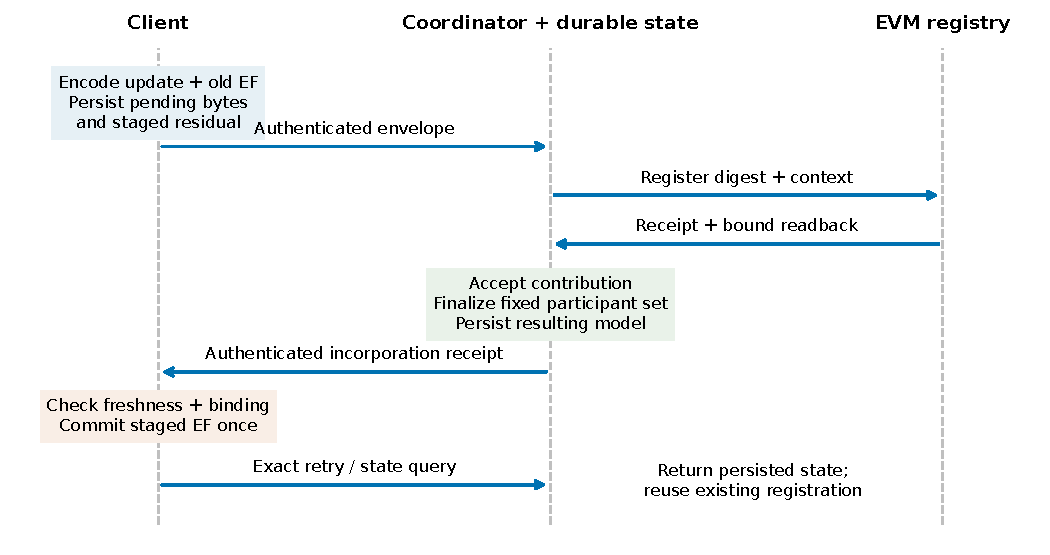
\includegraphics[width=0.9\linewidth]{revision_artifacts/v4_dualtrack/figures/figure3_upload_protocol.pdf}
\caption{An incorporation receipt connects chain registration to the next residual. Retries reuse persisted bytes and recover the recorded state before the client advances its generation.}\label{fig:uploadprotocol}
\end{figure}

\subsection{Recover the same update after an interrupted exchange}
A client reconstructs a retry from its persisted pending envelope. When registration succeeded before the response was lost, the coordinator retrieves that binding and continues acceptance; when aggregation finished before the response was lost, the coordinator returns the incorporated state and resulting-model digest. Reopening the service and client stores therefore resumes the existing record through the same receipt path.

Repeated acceptance, round finalization and residual commitment check their persisted states before applying a transition. While a round awaits its participant set, the coordinator retains the open round and model while clients retain pending updates and previous residuals. Recovery thus preserves one contribution and one residual-generation change per client--round, giving the upload history a direct interpretation in the learning state.
